\chapter{Løsninger til lineær programmeringsproblemer}
I dette kapitel vil forskellige typer af løsninger til lineære programmerings problemer blive gennemgået med udgangspunkt i \citep{bert}.
Gennemgangen har tilformål at undersøge, om de løsninger, hvis funktions værdi svare til den optimale værdi, (her refereret til som en optimal løsning), har nogle fællestræk som kan bruges til at udlede en løsnings metode.
Desuden undersøger kapitlet, hvornår der eksistere en optimal løsning.

\section{Basisløsninger}

%Jeg har endnu ikke fået gennemgået beviserne til de to sætninger ordentligt. de er bare stjålet fra jer andre.

Basisløsninger danner grundlaget for udregningen af den optimale løsning, hvilket beskrives og anvendes i Kapitel \ref{afsnit:simplex}. For at kunne beskrive netop basisløsninger er det nødvendigt først at introducere definitionen for aktive betingelser.%Ved ikke: Skal vi også bruge fed når ord introduceres i bindende tekst?

\begin{defn}[Aktive betingelser]
En betingelse siges at være en \textbf{aktiv betingelse} for en givet løsningsvektor $\vec{x}^*$, hvis det gælder, at\\ $\vec{a}_i^T \vec{x}^* = b_i$.
\label{def:aktiv}
\end{defn}

Generelt bliver aktive betingelser brugt, da de for uligheder repræsenterer en grænse for de mulige løsninger i en given retning, mens de for ligheder blot beskriver, at betingelsen er opfyldt.
Yderligere anvendes skæringen mellem disse aktive betingelser, da den optimale løsning for lineære programmeringsproblemer findes i netop disse skæringer. Hvorfor dette netop er tilfældet bliver begrundet i Afsnit \ref{sec:eksistens}.

\begin{stn}[Lineært uafhængige rækker]
Lad $\vec{x}^* \in \mathds{R}^n$ og $I = \{i | \vec{a_i}^T \vec{x}^* = b_i\}$ være mængden af indekser for aktive betingelser. Da er følgende udsagn ækvivalente:
\begin{enumerate}[label=(\alph*)]
\item Mængden $R_a =\{\vec{a_i}| i\in I\}$ indeholder vektorer, hvoraf $n$ af dem er lineært uafhængige.
\item Spannet $span(R_a) = \mathds{R}^n$.
\item Ligningssystemet $\vec{a_i}^T \vec{x}^* = b_i$, for $i \in I$ har en entydig løsning.
\end{enumerate}
\label{stn:uniklosning}
\end{stn} %Ved ikke: Bør det siges at $\vec{a_i}$ repræcentere en række, eller er det underforstået i rapporten da den altid gør det?

\begin{proof}
	(a) <=> (b): Antag at der i $R_a$ er $n$ lineært uafhængige vektorer. Da der er $n$ lineært uafhængige vektorer må dimensionen af spannet af $R_a$ være $n$. Da $dim(span(R_a))=dim(\mathds{R}^n)=n$ og da $R_a \subseteq \mathds{R}^n$ må det følge af Sætning \ref{stn:dimunderrum} at $span(R_a)=\mathds{R}^n$. Tilsvarende gælder det at hvis $span(R_a)=\mathds{R}^n$, må det gælde at $dim(span(R_a))=dim(\mathds{R}^n)=n$. Da vil kardinaliteten af en basis for $R_a$ nødvendigvis være $n$, hvorved $R_a$ skal indeholde $n$ lineært uafhængige vektorer.


(a) <=> (c): Antag at $span(R_a)=\mathds{R}^n$. Antag nu for modstrid, at der findes to løsninger, $\vec{x}_a$ og $\vec{x}_b$, som opfylder $\vec{a}_i\vec{x}=\vec{b}$ for alle $i \in I$. 
Da vil det for alle $i \in I$ gælde at $\vec{a}_i^T\vec{x}_a=\vec{b}$ og at $\vec{a}_i^T\vec{x}_b=\vec{b}$, hvorved $\vec{a}_i^T\vec{d}=\vec{0}$, hvor $\vec{d}=\vec{x}_a-\vec{x}_b$. 
Vektoren $\vec{d}$ vil da være orthogonal på alle $\vec{a}_i$ for $i \in I$ og kan derfor ikke være en lineær kombination af disse. Herved kan $R_a$ ikke udspænde hele $\mathds{R}^n$, da $\vec{d} \in \mathds{R}^n$ men $\vec{d} \notin span(R_a)$.
Tilsvarende antages det nu at der kun er en unik løsning til ligningssystemet. For modstrid antages det at $R_a$ ikke udspænder hele $\mathds{R}^n$ Der kan derved vælges en vektor $\vec{d}$ som er orthogonal til $span(R_a)$ hvorved $\vec{a}_i^T(\vec{x}+\vec{d})=\vec{b}$. Derved er $\vec{x}$ ikke en unik løsning og der er opstået modstrid.
\end{proof}
	
Nu hvor aktive betingelser og lineært uafhængige rækker er definere, kan basisløsninger definere og beskrives

\begin{defn}[Basisløsning og mulig basisløsning]
Lad $P$ være et polyeder dannet af lineære bibetingelser, og lad $\vec{x}^*\in \mathds{R}^n$. Da er $\vec{x}^*$ en \textbf{basisløsning}, hvis
\begin{enumerate}[label=(\alph*)]
\item Alle lighedskrav er aktive
\item Af de aktive betingelser er $n$ lineært uafhængige
\end{enumerate}
og en \textbf{mulig basisløsning}, hvis
\begin{enumerate}[label=(\alph*)]
\setcounter{enumi}{2}
\item hvis $\vec{x}^* \in P$ er en basisløsning.
\end{enumerate}
\label{def:basislosning}
\end{defn}
Det vil sige at en basisløsning ikke nødvendigvis ligger ikke i løsningsmængden, da skæringen mellem de $n$ lineært uafhængige krav ikke pr. Definition \ref{def:basislosning} behøver at ligge i løsningsmængden, og en mulig basisløsning er dermed det særtilfælde af basisløsninger som tilhører løsnings mængden.
En konsekvens af at en basisløsning altid skal have $n$ lineært uafhængige aktive betingelser er, i følge Sætning \ref{stn:uniklosning}, er at basisløsningen er en entydig løsning til ledningssystemet af de $n$ aktive bibetingelser.
%der skal måske lige laves en merge her
%Enhver bibetingelse udspænder et rum, for hvilket betingelsen er opfyldt. Skæringen, af de aktive betingelser, danner derved et rum, som er fællesmængden af betingelsernes udspændte rum. Skæringen, af en mængde af aktive betingelser, svarer derved til den mulige mængde af disse betingelser. Dog gælder det for basisløsninger pr. Definition \ref{def:basislosning}, at der for en basisløsning $\vec{x}$ skal være $n$ lineært uafhængige aktive betingelser, hvorved en basisløsningen er en unik vektor, hvilket er bevist igennem Sætning \ref{stn:uniklosning}. %Ved ikke, er en vektor og et punkt det samme?

\begin{kor}[Endelig mængde af basisløsninger]
Givet en endelig mængde af bibetingelser, vil der kun eksistere en endelig mængde af basisløsninger og derved også kun en endelig mængde mulige basisløsninger.
\label{kor:endeligbasis}
\end{kor}

\begin{proof}
Betragt et lineært ligningssystem med $m$ uligheder og løsningsvektorer på formen $\vec{x} \in \mathds{R}^n$, hvor m er et endeligt tal.
	Betragt da systemet af $n$ aktive uafhængige lineære uligheder udvalgt af de $m$ uligheder. Da vil dette system ifølge Sætning \ref{stn:uniklosning} kun have en løsning, og denne udvælgelse af uligheder giver derved kun en basisløsning. Da der kun er en endelig mængde af muligheder for at udtrække $n$ af $m$ uligheder på, vil der netop også kun være en endelig mængde af basisløsninger. Da mængden af mulige basisløsninger er en delmængde af mængden af basisløsninger, vil der også kun være en endelig mængde af mulige basisløsninger.
\end{proof}

Det at en basisløsning er en entydig løsning til ligningssystemet af dens $n$ lineært uafhængige bibetingelser kan bruges til at finde en procedure til at finde basisløsninger.

\begin{stn}[Krav til basisløsninger]
Lad $A\vec{x}=\vec{b}$ og $\vec{x}\geq 0$, hvor $A$ er en $m\times n$ matrix med lineært uafhængige rækker. Da er $\vec{x}^*\in \mathds{R}^n$ en basisløsning hvis og kun hvis $A\vec{x}^*=b, \vec{x}^* \geq 0$, og der eksisterer indekser $B(1), ..., B(m)$ således, at
\begin{enumerate}[label=(\alph*)]
\item Kolonerne $A_{B(1)}, ..., A_{B(m)}$ er lineært uafhængige og
\item $x_j = 0$, hvis $j \neq B(1),...,B(m)$.
\end{enumerate}
\label{stn:kravtilbasis}
\end{stn}

\begin{proof}
Først vises at (a) og (b) medfører at $\vec{x}$ er en basisløsning.
Lad $I_m$ være mængden af indeks for de lineært uafhængige søjler  $I_m=\{B(1),\dots,B(m)\}$. Per definition er $\vec{b}=\sum_{j=1}^{n} x_j \vec{A}_j$, hvilket må være det samme som $\vec{b}=\sum_{j\in I_m} x_j \vec{A}_j+\sum_{j\notin I_m} x_j \vec{A}_j$, hvor summeringen er opdelt efter om kolonnerne har indeks $i \in I_m$. 
Ifølge sætningens punkt (b) er $x_j=0$ for $j \notin I_m$. Derved bliver summeringen forkortet til $\vec{b}=\sum_{j\in I}x_j \vec{A}_j$. Da vektorerne $\vec{A}_j$ for $j \in I_m$ er lineært uafhængige vil ligningssystemet nødvendigvis have en unik løsning. Da ligningssystemet har en unik løsning gælder det af Sætning \ref{stn:uniklosning}, at ligningssystemet har $n$ lineært uafhængige rækker, som alle er aktive. Da der er $n$ aktive betingelser og da alle lighedskrav er aktive, vil det pr. Definition \ref{def:basislosning} sige at $\vec{x}$ er en basisløsning.

% som er summen af alle de lineære uafhængige rækker og deres løsninger lagt sammen med summen af de lineære afhængige rækker og deres løsninger, men $\vec{x_j}$ til de lineære uafhængige løsninger er er i følge sætningen $x_i = 0$ hvis $i \neq B(1),...,B(m)$ så derfor må ligningen blive $b=\sum_{j\in I_m}^{n}x_j \vec{A}_j+0$,
% 
%så derfor må $\vec{x}$ være en basis løsning.

Herefter vises at det at $\vec{x}$ er en basisløsning medfører (a) og (b). Antag at $\vec{x}$ er en basisløsning og lad $x_j$ for indekser $j \in I_k=\{B(1),\dots B(k)\}$ være alle ikke-nul komponenter af $\vec{x}$.
Eftersom $\vec{x}$ er en basisløsning, så må ligningssystemet af aktive betingelser $\sum_{j=1}^{n}\vec{A}_jx_j=\vec{b}$, hvor $x_j=0$ for $j\notin I_k$ have en unik løsning. Dette gælder da en basisløsning har $n$ lineært uafhængige aktive betingelser, hvilket ifølge Sætning \ref{stn:uniklosning} medfører at systemet har en unik løsning. 
Ligeledes må ligningen $\sum_{j \in I_k}\vec{A}_jx_j=\vec{b}$ have en unik løsning og derfor må kolonerne $\vec{A}_{B(1)}, ..., \vec{A}_{B(k)}$ være lineært uafhængige. Derfor må det gælde at $k \leq m$. % Hvis ikke dette var tilfældet ville der eksistere flere $\vec{x}$ som opfylder ligningssystemet, hvilket modstrider at der er en unik løsning.\\
%Eftersom kolonerne $\vec{A}_{B(1)}, ..., \vec{A}_{B(k)}$ er lineært uafhængige, så må det gælde at $k\leq m$. 
Da $A$ har $m$ lineært uafhængige rækker, må $A$ også have $m$ lineært uafhængige kolonner, hvorved $Col(A)=\mathds{R}^m$.

Den næste del af beviset viser, at der for enhver udvælgelse af indekser $I_k$ findes indekser $I_m$ således at $I_k \subseteq I_m$. 
%Den næste del af beviset viser, at der for enhver udvælgelse af $k$ lineært uafhængige kolonner med indekser $I_k$, gælder at der findes en mængde af $m$ lineært uafhængige kolonner med indekser $I_m$, hvorom det gælder at $I_k \subseteq I_m$.
Altså findes der indekser $B(k+1),...,B(m)$, således at kolonnerne med indekser $B(1),...,B(k),...,B(m)$ er lineært uafhængige. 

Hvis alle $\vec{A}_j$ for $j \notin I_k$ er lineært afhængige af $\vec{A}_j$ for $j \in I_k$, gælder det at $span\left( \vec{A}_{B(1)},...,\vec{A}_{B(k)} \right)=Col(A)=\mathds{R}^m$, hvorved $k=m$. 
Hvis der i stedet eksisterer en kolonne med indeks $j \notin I_k$ som er lineært uafhængig af disse kolonner, kan denne tilføjes til mængden af nu $k+1$ uafhængige vektorer. Denne proces kan gentages $m-k$ gange. Da $i \notin I_m$ medfører at $i \notin I_k$ gælder det derved at $\vec{x}_i =0$ for $i \notin I_m$
\end{proof}

\begin{pro}{Procedure for konstruktion af basisløsninger}
Vælg $m$ lineært uafhængige koloner $\vec{A}_{B(1)},\dots,\vec{A}_{B(m)}$
Lad $x_i=0 \,\forall i\neq B(1),\dots,B(m)$
Løs $A\vec{x}=\vec{b}$ for de ubekendte $x_{B(1)},\dots x_{B(m)}$
\end{pro}
Bemærk at proceduren indirekte kan bruges til at finde mulige basisløsninger, da de er et særtilfælde af basisløsninger.\\
%En Basis løsning lavet med denne procedure, så længde den ikke er negativ, kaldes den for en mulig basisløsning. Og fordi en mulig basisløsning er en basisløsning, så kan en mulig basisløsning findes, ved at lave basisløsninger.\\

Hvis $\vec{x}$ er en basisløsning, kaldes indgangene $x_{B(1)},\dots ,x_{B(m)}$ for basis variable, mens $x_i \,\forall i\neq B(1),\dots,B(m)$ kaldes for ikke-basis variabler. Mens søjlerne $\vec{A}_{B(1)},\dots,\vec{A}_{B(m)}$ udgør en basis for $\mathds{R}^m$ ifølge Sætning \ref{stn:uniklosning}.
\begin{defn}
Lad $\vec{x}$ en basisløsning så $x_i = 0$ for alle $i \notin I_B$, da er $B = [\vec{A_i}: i \in I_B]$ \textbf{basismatricen} knyttet til basisløsningen. 
Og ved $\vec{x}_B$ forstås løsningen til ligningsstemmet $B\vec{x}_B =\vec{b}$.
\end{defn}
Bemærk at da $B$ består af $m$ lineært uahængige rækker og er en $m\times m$ matrix følger det af Sætning \ref{stn:inversmatrix}, at $B^{-1}$ eksistere. 


%\\ %måske et andet ord
%Søjlerne $A_{B(1)},\dots ,A_{B(m)}$ kaldes for basis søjlerne og da de er lineært uafhængige, så danne de en basis for $\mathds{R}^m$\\
%To baser kan være forskellige, men de vil blive betragtet som værende to forskellige mængder $\{B(1),\dots,B(m)\}$ af basis indekser, hvis disse to mængde består af de samme basis indekser, så vil de blive betragtet som værende samme basis.\\
%Hvis søjlerne $\vec{A}_{B(1)},\dots,\vec{A}_{B(m)}$, bliver sat ved siden af hinanden, så der dannes $m\times m$ matrixen $B$, som kaldes en basis matrix. ligeledes dannes vektoren $\vec{x}_{B}$ bestående af basis variablerne. Basis variablerne er bestemt ved at løse ligningen $B\vec{x}_B=\vec{b}$ således at en unik løsning er givet ved $\vec{x}_B=B^{-1}\vec{b}$
%\begin{defn}
%Betragt en $m\times m$ basis matrix $B$ dannet af lineært uafhængige søjler fra $A$ i $A\vec{x}=\vec{b}$
%
%\end{defn}

\begin{comment}
Der mangler bare generelt bindetekst mellem sætninger, fra at korollar 6.12 skal introduceres til at kapitlet skal afsluttes og føres videre til naboløsninger
\end{comment}





\subsection{Naboløsninger}

Til den senere anvendelse af simplex metoden anvendes også \textbf{naboløsninger}, som er defineret i Definition \ref{def:nabo}. Undersøgelsen af naboløsninger i simplex metoden som en metode til at reducere antallet af basisløsninger, som skal undersøges når den optimale løsning findes. %Bør omformuleres, er kringlet. Ved ikke: Er det realt det der sker? Ved ikke: Skal SimpLeX staves med stort? Jeg tror da det er det der sker. og simplex er med lille. hermed rettet.

\begin{defn}[Naboløsninger]
	To basisløsninger i $\mathds{R}^n$ siges af være \textbf{naboløsninger}, hvis de deler præcis $n-1$ aktive lineært uafhængige bibetingelser.
	\label{def:nabo}
\end{defn}

Et eksempel på naboløsninger ses i Eksempel \ref{eks:nabo}.

\begin{eks}[Naboløsninger]
De to basisløsninger $\vec{p}=\rvect{4 & 4}^T$ og $\vec{q}=\rvect{10 & 2}^T$ set på Figur \ref{fig:nabo} er naboløsninger, da de har $n-1$ fælles aktive betingelser, hvilket for dette eksempel er $1$ betingelse, nemlig betingelse (2). Basisløsningen $\vec{p}$ har (1) og (2) som aktive betingelser, mens $\vec{q}$ har (2) og (3) som aktive betingelser. %ved ikke, om nemlig bør slettes.
	
	\begin{center}
	\begin{tabular}{l	>{$}r<{$}	>{$}r<{$}	>{$}l<{$} r}
	Maksimer 		& 		4x_1	&	+3 x_2	& \\
	med hensyn til 	&  \ \ 	-2 x_1	& 	+4 x_2	& \leq 8 	& \quad (1)\\
					&  		x_1		& 	+3 x_2	& \leq 16	& \quad (2)\\
					&  \ \ 	x_1		& 			& \leq 10	& \quad (3)\\
	og $x_1 \geq 0$ (4), $x_2\geq 0$ (5).
	\end{tabular}
	\end{center}
	
	\begin{center}
	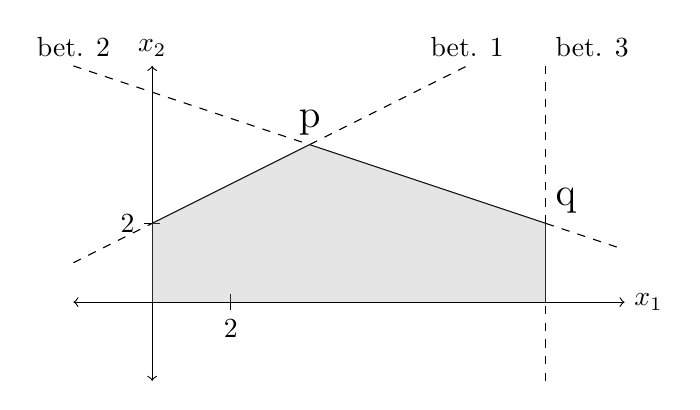
\begin{tikzpicture}
  %laver Grid. godt til når koordinater skal redigeres
  	%\draw[thin,gray!40] (-3,-1) grid (6,3); 
  %x-aksen
  	\draw[<->] (-1,0)--(6,0) node[right]{$x_1$};
  	%\draw[->,red] (2.5,0) -- (2.5,0.5);
  %y-aksen
  	\draw[<->] (0,-1)--(0,3) node[above]{$x_2$};
  	%\draw[->,red] (0,0.5) -- (0.5,0.5);
  	
  %akse-markeringer
  	%\node[left] (xakse) at (0,1) {2};
  	\draw[] (-0.1,1) -- (0.1,1) node[pos=0,left] {2};
  	\draw[] (1,-0.1) -- (1,0.1) node[pos=0,below] {2};
  	
  %ligning 1
	\draw[domain=-1:0,variable=\x,dashed] 	plot({\x},{0.5*\x+1});
	\draw[domain=0:2,variable=\x] 			plot({\x},{0.5*\x+1});
	\draw[domain=2:4,variable=\x,dashed] 	plot({\x},{0.5*\x+1}) node[above] {bet. 1};
  	%\draw[->,red] (1,1.5) -- (1.224,1.05);
	
  %ligning 2
  	\draw[domain=-1:2,variable=\x,dashed] 	plot({\x},{-(1/3)*\x+8/3}) node[above] at (-1,3) {bet. 2} ;
	\draw[domain=2:5,variable=\x] 			plot({\x},{-(1/3)*\x+8/3});
	\draw[domain=5:6,variable=\x,dashed] 	plot({\x},{-(1/3)*\x+8/3});
	%\draw[->,red] (3.5,1.5) -- (3.34,1.026);

  %ligning 3
  	\draw[domain=-1:0,variable=\y,dashed] 	plot({5},{\y});
	\draw[domain=0:1,variable=\y] 			plot({5},{\y});
	\draw[domain=1:3,variable=\y,dashed] 	plot({5},{\y}) node[above right] {bet. 3};
	%\draw[->,red] (5,0.5) -- (4.5,0.5);

  %nodes med navne på punkter
	\node[above] (p) at (2,2) {\Large p};
	\node[above right] (q) at (5,1) {\Large q};

  %løsningsmængden skraveret
	\fill[gray!80,nearly transparent] (0,0) -- (0,1) -- (2,2) -- (5,1) --(5,0) --  cycle;
\end{tikzpicture}
	\captionof{figure}{Løsningsmængde med naboløsninger $p$ og $q$.}
	\label{fig:nabo}
	\end{center}
	
\label{eks:nabo}
\end{eks}

%ved ikke: Må et afsnit slutte med et eksempel?
\subsection{Degenererede basisløsninger}
En basisløsning skal have $n$ aktive lineært uafhængige bibetingelser i følge Definition \ref{def:basislosning} (b), det udelukker ikke at en basisløsning kan have flere aktive krav, hvis nogle af kravende er lineært afhængige. 
\begin{defn}[Degenereret basisløsning]
En basisløsning $\vec{x}\in \mathds{R}^n$ siges at være en \textbf{degenereret basisløsning}, hvis basisløsningen har mere en $n$ aktive bibetingelser.
\end{defn}
Det vil sige, at for $\vec{x}\in \mathds{R}^2$, vil $\vec{x}$ være degenereret, hvis $\vec{x}$ ligger på et skæringspunkt af $3$ bibetingelser.
Af Sætning \ref{stn:PQ} følger det, at antagelsen om, at alle bibetingelser er lineært uafhængige ikke ændre løsningsmængden, derfor vil denne rapport kun meget overfladisk nævne degenererede løsninger. 
Men da degenerede løsninger kan give nogle problematikker senere i Simplex metoden, så den terminerer for tidligt, defineres degenererede basisløsninger, for at vise en forståelse for emnets eksistens.
Helt generelt gælder der for basisløsninger til et polyeder på standard form med ligheder, at der altid vil $m$ lighedsbetingelser  aktive. Derfor må, det at have mere end $n$ aktive bibetingelser, betyde at mere end $n-m$ variabler er $0$
\begin{defn}
Lad $P =\{ \vec{x} \in \mathds{R}^n \mid A \vec{x} = \vec{b}, \, \vec{b}\in \mathds{R}^m\}$ være et polyeder på standard form med ligheder, og lad $\vec{x}$ være en basisløsning. Lad $m$ være mængden af rækker i $A$. Så er $\vec{x}$ en degenereret basisløsning, hvis mere end $n-m$ komponenter af $\vec{x}$ er $0$.
\end{defn}


%I følge af definition \ref{def:basislosning} (b) skal en basis løsning, bare have $n$ lineære uafhængige aktive betingelser i $\mathds{R}^n$, dette giver muligheden for, at der er mere end $n$ aktive betingelser (Der kan selvfølge i $\mathds{R}^n$ ikke være mere end $n$ lineære uafhængige aktive betingelser). Sådan en basisløsning kaldes for en Degenereret basisløsning. Der vil i denne rapport, ikke blive arbejdet med degenereret basisløsninger, da der menes at rapports indhold i forvejen er tilstrækkeligt, dette kan komme til at give nogle problematikker senere i Simplex-metoden, der for den til at terminere for tidligt, så derfor defineres degenereret basisløsninger, for at vise en forståelse for emnet eksistens.
%\begin{defn}[Degenereret basisløsning]
%En basisløsning $\vec{x}\in \mathds{R}^n$ siges at være en \textbf{Degenereret basisløsning}, hvis basisløsningen har mere en $n$ aktive betingelser
%\end{defn}

%Det vil sige, at for $\vec{x}\in \mathds{R}^2$, vil $\vec{x}$ være degenereret, hvis $\vec{x}$ ligger på et skæringspunkt af $3$ betingelser.
%\textit{måske et eksempel}\\
%\subsubsection{Degenereret basisløsninger i standard form}
%En basisløsning til en polyede på standard form, vil $m$ lighedsbetingelser altid være aktive. Derfor må, at have mere end $n$ aktive betingelser, være at mere end $n-m$ variabler er $0$
%\begin{defn}
%En polyede på standard form $P =\{ \vec{x} \in \mathds{R}^n | A \vec{x} = \vec{b}, \vec{b}\in \mathds{R}^m\}$ og lad $\vec{x}$ være en basisløsning. Lad $m$ være mængden af rækker i $A$. Så er $\vec{x}$ en degenereret basisløsning, hvis mere end $n-m$ komponenter af $\vec{x}$ er $0$
%\end{defn}
%Dette vil dog næsten ikke ske, hvis komponenterne af $A$ og $\vec{b}$ er valgt tilfældigt.
%Det der sker er, at når der bliver valgt $m$ rækker af $A$ som danner basis og $m$ variabler bliver udregnet til en basisløsning, så opfylder denne løsning også et andet krav, og derfor vil der under rækkeoperationerne resultere i, at en af de valgte variabler bliver $0$
\section{Eksistens af en optimale løsning}
\label{sec:eksistens}
Hvis det lineære programmeringsproblem er konsistent, betyder det, at der er en løsning til det, men bare fordi der er en løsning, betyder det ikke, at der er en optimal løsning.
Hvis der skal eksistere en optimal løsning, må løsningsmængden ikke indeholde en linje.
%\begin{defn}[Linje]
%Lad $P\subseteq \mathds{R}^n $ være et polyeder, da indeholder $P$ en \textbf{linje}, hvis $\vec{x}+\lambda\vec{d} \in P$ for alle $\lambda \in \mathds{R}_+$, hvor $\vec{x}\in P$ og $\vec{d} \in \mathds{R}^n$. Hvis $\vec{x}+\lambda\vec{d} \in P$ for $\lambda > 0$ eller $\lambda < 0$, siges $P$ at indeholde henholdsvis en positiv eller negativ halv linje.
%
%\end{defn}

\begin{defn} [Linje]
Lad $P\subseteq \mathds{R}^n $ være et polyeder og $\vec{x} \in P$, da indeholder $P$ ikke en \textbf{positiv halvlinje}, hvis $\forall \vec{d} \in \mathds{R}^n \nexists \lambda \in \mathds{R}_+ : \vec{x}+\lambda \vec{d} \in P$, og indeholder ikke en \textbf{linje} hvis $\forall \vec{d} \in \mathds{R}^n \nexists \lambda \in \mathds{R} : \vec{x}+\lambda \vec{d} \in P$.
\label{def:linje}
\end{defn}

Det betyder, at der til en løsning i polyederet kan lægges en retningsvektor til.
Denne retningsvektor bliver skaleret, så løsningen nu ligger et andet sted. 
Hvis der findes en retning, hvor det resulterer i at løsning stadig er i polyeden, selvom $\lambda$ er vilkårligt stor, så siges polyederet at have en linje.
%Det betyder, at der til en løsning kan lægges et vilkårligt stort multiplum af en vektor til, og summen vil stadig være en løsning, derfor må objektfunktionen nødvendigvis også kunne tage en vilkårlig stor værdi.
\begin{prop}
Lad løsningsmængden $P = \{ \vec{x} \in \mathds{R}^n\mid A \vec{x} \geq \vec{b} \} \subseteq \mathds{R}^n $  til det lineære minimeringsproblem $\vec{c}^T\vec{x}$, indeholde en linje
\begin{align*}
\vec{x} + \lambda \vec{d}, \quad \vec{d}\in \mathds{R}^n, \, \vec{c}^T\vec{x} \neq 0, \, \lambda \in \mathds{R}.
\end{align*}
Da er den optimale værdi $-\infty$.
\end{prop}
\begin{proof}
Da $P$ indeholder en linje, følger det af Definition \ref{def:linje}, at der eksistere en vektor $\vec{x} \in P$ og en vektor $\vec{d} \in \mathds{R}^n$, så $\vec{x}+\lambda \vec{d} \in P$, for alle $\lambda \in \mathds{R}^n$. 
Fordi $\vec{c}^T\vec{d}\neq 0$, medfører det, at $\lambda$ kan vælges så $\vec{c}^T(\vec{x}+\lambda\vec{d}) = - \infty$, hvorfor den optimale værdi må være $-\infty$.
\end{proof}
Bemærk, at da løsningsmængden indeholder en linje, kan løsningsmængden ikke være tom, er løsningsmængden tom, er problemet inkonsistent, og der eksistere derfor ikke en optimal løsning. 
Er løsningsmængden ikke tom, og uden linjer, da eksistere der en optimal løsning, som viser sig at være en mulig basisløsning.
\begin{stn}[Eksistens af en optimal løsning]
Hvis løsningsmængden $P =\{\vec{x} \in \mathds{R}^n\mid A \vec{x} \geq \vec{b} \} \neq \emptyset$, til det lineære minimeringsproblem $\vec{c}^T\vec{x}$, ikke indeholder en positiv halvlinje, da vil der eksistere en optimal løsning $\vec{x}^{**}$, som er en mulig basisløsning.
\label{stn:eksistens}
\end{stn}
\begin{proof}
Antag, at $\vec{x} \in P$ ikke er en mulig basisløsning, og lad $I =\{i \mid \vec{a_i}^T\vec{x}=b_i\}$ betegne indeksene for de lineært uafhængige aktive bibetingelser knyttet til løsningen $\vec{x}$.
Da $\vec{x}$ ikke er en mulig basisløsning, må $span(\{\vec{a_i}\mid i\in I\})$ være et ægte underrum til $\mathds{R}^n$, hvormed det følger af Sætning \ref{stn:Rnorto}, at der eksisterer en vektor $\vec{d} \in \mathds{R}^n$, så $\vec{a_i}^T\vec{d}=0$ for $i \in I$.
Da må $\vec{a_i}^T(\vec{x}\pm \vec{d})= \vec{a_i}^T\vec{x}=b_i$.
Vælg nu fortegn på $\vec{d}$ så $\vec{c}^T\vec{d}\leq 0$, da må $\vec{c}^T(\vec{x}+\lambda\vec{d}) \leq \vec{c}^T\vec{x}$ for en vilkårlig skalar $\lambda > 0$.
Da løsningsmængden ikke indeholder en positiv halvlinje, vil der være en øvre grænse for $\lambda$, før $\vec{x}+\lambda\vec{d} \notin P$, svarende til $\lambda$et, der opfylder $\vec{a_j}^T(\vec{x}+\lambda\vec{d})=b_j$, hvor $\vec{a_j} \notin \{\vec{a_i}\mid i\in I\}$ er den første bibetingelse, der bliver aktiv, se Figur \ref{fig:eksistens}.
Da $\vec{a_i}^T\vec{d}=0$ og $\vec{a_j}^T\vec{d} \neq 0$ medfører det, at $\vec{a_i}$ og $\vec{a_j}$  er lineært uafhængige af Lemma \ref{lma:ortolinuaf}. 
Derfor kan $j$ tilføjes til $I$.
Gentag til at $|I|=n$.
\\ Antag nu, at $|I|=n$, derfor må $\vec{x}$ have $n$ aktive bibetingelser.
Da $\vec{x}\in \mathcal{F}$ medfører det, at $\vec{x}$ overholder alle ligheds bibetingelser, og at $\vec{x}$ er en mulig løsning. 
Derfor følger det af Definition \ref{def:basislosning}, at $\vec{x}$ er en mulig basisløsning.
\\Derfor må der fra en vilkårlig løsning $\vec{x}\in \mathcal{F}$ kunne konstrueres en mulig basisløsning $\vec{x^*}$ så $\vec{c}^T\vec{x^*} \leq \vec{c}^T \vec{x}$.
Dermed må den optimale løsning være den mulige basisløsning, der minimere objektfunktionen, hvorfor der eksistere en optimal løsning, som er en mulig basisløsning.
\end{proof}
\begin{figure}
\begin{center}
	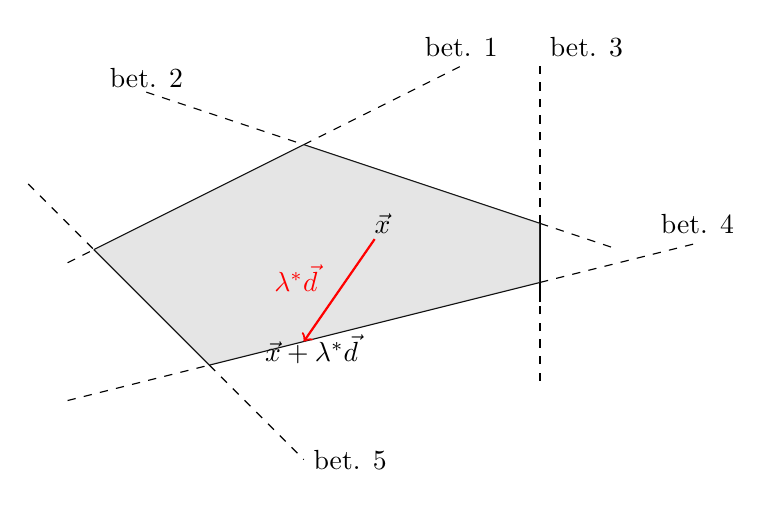
\begin{tikzpicture}[ latex
  s/.style={width=0}]

  %ligning 1
	\draw[domain=-1:-2/3,variable=\x,dashed] 	plot({\x},{0.5*\x+1});
	\draw[domain=-2/3:2,variable=\x] 			plot({\x},{0.5*\x+1});
	\draw[domain=2:4,variable=\x,dashed] 	plot({\x},{0.5*\x+1}) node[above] {bet. 1};
	
  %ligning 2
  	\draw[domain=0:2,variable=\x,dashed] 	plot({\x},{-(1/3)*\x+8/3}) node[above] at (0,2.6) {bet. 2} ;
	\draw[domain=2:5,variable=\x] 			plot({\x},{-(1/3)*\x+8/3});
	\draw[domain=5:6,variable=\x,dashed] 	plot({\x},{-(1/3)*\x+8/3});
	

  %ligning 3
  	\draw[domain=-1:0,variable=\y,dashed] 	plot({5},{\y});
	\draw[domain=0:1,variable=\y] 			plot({5},{\y});
	\draw[domain=1:3,variable=\y,dashed] 	plot({5},{\y}) node[above right] {bet. 3};
	
  %ligning 4
	\draw[domain=-1:4/5,variable=\x,dashed] 	plot({\x},{0.25*\x-1});
	\draw[domain=4/5:5,variable=\x] 			plot({\x},{0.25*\x-1});
	\draw[domain=5:7,variable=\x,dashed] 	plot({\x},{0.25*\x-1}) node[above] {bet. 4};
	
  %ligning 5
  	\draw[domain=-1.5:-2/3,variable=\x,dashed] 	plot({\x},{-\x}) ;
	\draw[domain=-2/3:4/5,variable=\x] 			plot({\x},{-\x});
	\draw[domain=4/5:2,variable=\x,dashed] 	plot({\x},{-\x}) node[right] {bet. 5} ;

  %løsningsmængden skraveret
	\fill[gray!80,nearly transparent] (4/5,-4/5) -- (-2/3,2/3) -- (2,2) -- (5,1) --(5,0.25) --  cycle;
	
  % vektor x
	\node[] (x) at (3,1) {$\vec{x}$};
	\draw[thick, color=red, ->](2.9,0.8) -- (2,-0.5) node[above, yshift=0.5 cm, xshift=-0.1 cm] {$\lambda^* \vec{d}$} ;
	\node[] (x) at (2.1, -0.6) {$\vec{x}+\lambda^* \vec{d}$};
 
\end{tikzpicture}
	\captionof{figure}{Der ligges et multiplum af en retnings vektor til vektor $\vec{x}$ til at summen gør betingelse $4$ aktiv.}
	\label{fig:eksistens}
\end{center}
\end{figure}
Det betyder at hvis det lineære programmerings problem er konsistent, da eksistere der enten en optimal løsning, blandt basisløsningerne eller den optimale løsning er $\pm \infty$.
Det kunne derfor være relevant at finde en måde, hvor den optimale løsning blandt basisløsningerne kan findes, her kan gøres brug af simplex metoden.




\subsection{Lokal optimal løsning}
Når først en optimal løsning er fundet, er det nødvendigt at tjekke, at der ikke er tale om en lokal optimal løsning.
\begin{defn}[Lokalt optimal løsning]
Lad $\vec{x} \in P$ være en løsnings til et minimeringsproblem med objektfunktion $f$, da er $\vec{x}$ en \textbf{lokal optimal løsning}, hvis der for en naboløsning $\vec{y}$ gælder, at $f(\vec{x}) \leq f(\vec{y})$ for $|\vec{y}-\vec{x}|< \epsilon$ for et $\epsilon > 0$ og $\vec{y} \in P$.
\end{defn}
Betragt beviset for Sætning \ref{stn:eksistens}, her konstrueres hele tiden en mere optimal løsning end den foregående, ved at lægge et multiplum af en retningsvektor til den originale vektor, så en ny betingelse blev aktiv.
Der vil derfor kunne opstå et lokalt minimum, hvis der ikke eksistere en sådan retningsvektor, men der er en løsning som er mere optimal, se Figur \ref{fig:lokaltmin}.
\begin{figure}
\begin{center}
	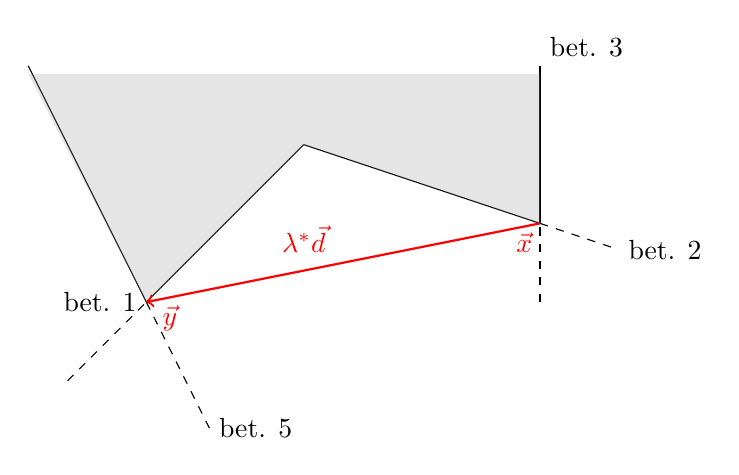
\begin{tikzpicture}[ latex
  s/.style={width=0}]

  %ligning 1
	\draw[domain=-1:0,variable=\x,dashed] 	plot({\x},{\x})  node[left] {bet. 1};
	\draw[domain=0:2,variable=\x] 			plot({\x},{\x});

	
  %ligning 2
	\draw[domain=2:5,variable=\x] 			plot({\x},{-(1/3)*\x+8/3});
	\draw[domain=5:6,variable=\x,dashed] 	plot({\x},{-(1/3)*\x+8/3}) node[right] {bet. 2};
	

  %ligning 3
	\draw[domain=0:1,variable=\y, dashed] 			plot({5},{\y});
	\draw[domain=1:3,variable=\y] 	plot({5},{\y}) node[above right] {bet. 3};
	

	
  %ligning 5
  	\draw[domain=-1.5:0,variable=\x] 	plot({\x},{-2*\x}) ;
	\draw[domain=-0:4/5,variable=\x, dashed] 			plot({\x},{-2*\x}) node[right] {bet. 5} ;


  %løsningsmængden skraveret
	\fill[gray!80,nearly transparent]  (0,0) -- (2,2) -- (5,1) -- (5,2.9) --(-1.5,2.9) --  cycle;
	
  % vektor x
  \node[thick, color=red] (x) at (4.8,0.75) {$\vec{x}$};
  
\node[thick, color=red] (y) at (0.3,-0.2) {$\vec{y}$};
%   %\node[s] (d) at (2, -0.5);
 \draw[thick, color=red, ->](5,1) -- (0,0) node[above, yshift=0.5 cm, xshift=2 cm] {$\lambda^* \vec{d}$} ;
%   \node[] (x) at (2.1, -0.6) {$\vec{x}+\lambda^* \vec{d}$};
%  % \path (x) edge node[right] {$\vec{x}+\lambda^* \vec{d}$} (d) ;
 
\end{tikzpicture}
	\captionof{figure}{Bemærk at der ikke eksistere en retningsvektor $\vec{d}$, så der kan konstueres en bedre løsning, uden at overskride betingelse $2$, derfor vil løsningsvektor $\vec{x}$ fremstå optimal, selvom at løsningsvektor $\vec{y}$ er mere optimal. Løsningsvektor $\vec{x}$ er et lokalt minimum.}
	\label{fig:lokaltmin}
\end{center}
\end{figure}
Det er dog ikke alle mængder, hvor der kan forekomme lokale optimale løsninger, ved fremgangsmåden fra beviset for Sætning \ref{stn:eksistens}.
\begin{defn} [Konveks mængde]
Lad $S \subset \mathds{R}^n$  da er $S$ konveks, hvis der $\forall \vec{x}, \vec{y} \in S$ og et vilkårligt $\lambda \in [0,1]$ gælder at $\lambda \vec{x} + (1-\lambda) \vec{y} \in S$.
\label{def:Konveks}
\end{defn}
En konveksmængde er en mængde der opfylder at det vægtede gennemsnit af et hvert par af elementer også tilhører mængden, det betyder at der altid kan findes en retningsvektor mellem et hvert punkt i mængden.
Helt generelt gælder det, hvis løsningsmængden til et lineært ligningsproblem er konveks, så vil en hver lokal optimal løsning, være en optimal løsning.
\begin{stn}
Lad $\vec{x} \in P$ være en lokal optimal løsnings til et lineært programerignsproblem  med objektfunktion $f$.
Da er  $f(\vec{x}) \leq f(\vec{y})$ for alle $\vec{y} \in P$ hvis $P$ er konveks.
\end{stn}
\begin{proof}
Antag at $\vec{x}^* \in P$ er en optimal løsning.
Da $P$ er konveks medfører det at $\lambda \vec{x}^* + (1-\lambda)\vec{x} \in P$. 
Da $\lambda$ kan vælges til at være vilkårligt tæt på nul, må $|\lambda \vec{x}^* + (1-\lambda)\vec{x} - \vec{x}| < \epsilon$ da
\begin{align*}
 |\lambda \vec{x}^* + (1-\lambda)\vec{x} - \vec{x}| = | \lambda \vec{x}^* - \lambda\vec{x}| = \lambda|\vec{x}^* - \vec{x}| < \epsilon.
\end{align*}
Da $\vec{x}$ er en lokal optimal løsning, følger det, at
\begin{align*}
f(\vec{x}) \leq f(\lambda \vec{x}^* + (1-\lambda)\vec{x}).
\end{align*}
Da $f$ er lineær følger det af Definition \ref{def:linfunk}, at 
\begin{align*}
f(\vec{x}) \leq f(\lambda \vec{x}^* + (1-\lambda)\vec{x}) &= \lambda f(\vec{x}^*) + (1-\lambda)f(\vec{x}) \qquad \Rightarrow
\\ f(\vec{x}) - f(\vec{x}) &=\lambda f(\vec{x}^*) + (1-\lambda)f(\vec{x}) \qquad \Rightarrow
\\ 0 & = \lambda( f(\vec{x}^*) - f(\vec{x})),
\end{align*}
hvis $\lambda$ er lille nok.
Da $ \lambda$ kan være forskellig fra nul må det medføre, at $f((\vec{x}^*) - f(\vec{x}) = 0$, hvorfor $f(\vec{x}^*) =f(\vec{x})$. 
Det kan derfor konkluderes, hvis $\vec{x}$ er en lokal optimal løsning, så er $\vec{x}$ en optimal løsning.
\end{proof}
Løsningsmængden  for et standard problem, vil altid være konveks.
\begin{stn}
Lad $P =\{ \vec{x} \in \mathds{R}^n | A \vec{x} \geq \vec{b}\} $ være en polyede, da er $P$ konveks.
\label{stn:polykon}
\end{stn}
\begin{proof}
Lad $\vec{x}, \vec{y} \in P=\{ \vec{x} \in \mathds{R}^n | A \vec{x} \geq \vec{b}\}$ være to vilkårlige vektorer, da gælder at $A\vec{x} \geq \vec{b}$ hvilket medfører at $\lambda A \vec{x} \geq \lambda\vec{b}$, hvor $\lambda \in [0,1]$ er en skalar. 
På ligefod må der derfor gælde at $(1-\lambda)A\vec{y} \geq (1-\lambda)\vec{b}$.
De to uligheder adderes nu
\begin{align*}
\lambda A \vec{x} + (1-\lambda) A \vec{y} \geq \lambda \vec{b} + (1 - \lambda) \vec{b}
\\  A (\lambda\vec{x} + (1-\lambda)\vec{y}) \geq \vec{b}.
\end{align*}
Derfor må $\lambda\vec{x} + (1-\lambda)\vec{y} \in P$.
\end{proof}
Det betyder derfor at et hvert lineært programmerings problem kun har optimale løsninger, da det er vist i Kapitel \ref{Afsnit:LinProg}, hvordan ethvert lineært programmerings problem kan skrives på standard form.

